\section{Stockage des boîtes et visualisation}\label{sec:vis}

\subsection{\'Etude d'une solution possible : le QuadTree}{\color{red} À discuter}
\paragraph{}Une des solutions qui pourrait permettre une visualisation fluide du pavage tout en répondant au document de spécifications serait de représenter le pavages sous une forme de QuadTree pour deux dimensions ou OcTree pour trois dimensions.
\begin{figure}[htbp]
\centering
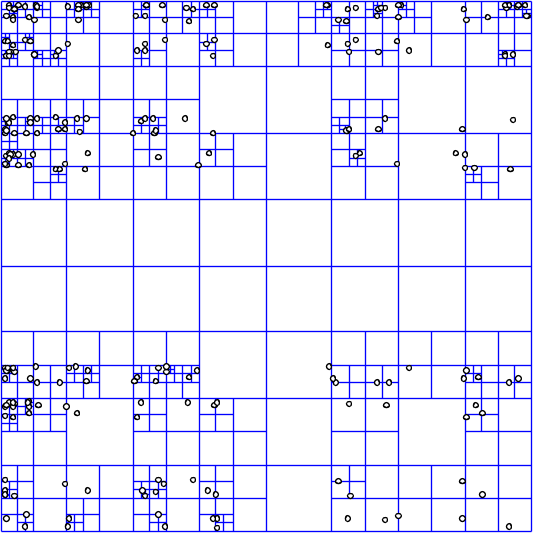
\includegraphics[scale=0.50]{img/quadtree}
\caption{Représentation d'un QuadTree où les données sont des points}

\end{figure}

Le QuadTree consiste à découper récursivement un espace fini en deux dimensions en quatre parties égales. Chacune de ces parties sont stockées dans une cellule. On itère ce mécanisme sur chacune de ces cellules jusqu'à isoler spatialement les éléments recherchés.
Cette structure pourrait être utilisée pour déterminer la position des boîtes dans l'espace.

\paragraph{}L'algorithme permettant de partitionner est récursif. Dans le cas récursif, l'algorithme divise une cellule en quatre et itère sur chacune des sous cellules. Dans le cas d'arrêt on ne subdivise plus. Nous décrivons par la suite l'ensemble des cas de récursions et d'arrêts pour la division d'une cellule donnée. Les images jointes au texte sont des représentations des différents cas dans lesquels les cadres rouges sont des boîtes solutions et les cadres noirs une cellule du QuadTree. Vous trouverez une classification visuelle dans la table \ref{tab:algo}.
\begin{enumerate}
\item Cas d'arrêts : 
\begin{enumerate}
\item La cellule fournie est entièrement inclus dans une boîte.
\label{enu:quad1}
\item La cellule fournie contient entièrement une seule boîte.
\label{enu:quad2}
\item La cellule fournie contient en partie une seule boîte.
\label{enu:quad3}
\item La cellule fournie n'intersecte aucune boîte.
\label{enu:quad4}
\item La cellule fournie ne peux plus être subdivisé car on a fourni une taille minimale pour les espaces.
\end{enumerate}
\item cas de récursions :
\begin{enumerate}
\item La cellule fournie intersecte plusieurs boîtes.
\label{enu:quad5}
\end{enumerate}
\end{enumerate}

\begin{table}[htbp]
\centering
 \begin{tabular}{|c|cccc|}
  \hline
  Cas de récursion &  \ref{enu:quad5}.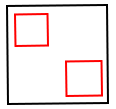
\includegraphics[scale=0.20]{img/QT4}&  \ref{enu:quad5}.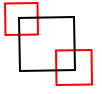
\includegraphics[scale=0.20]{img/QT5}& &\\
  \hline
  Cas d'arrêt&  \ref{enu:quad1}.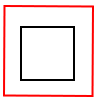
\includegraphics[scale=0.20]{img/QT1}&  \ref{enu:quad2}.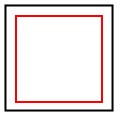
\includegraphics[scale=0.20]{img/QT2}&  \ref{enu:quad3}.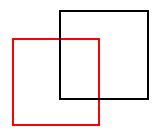
\includegraphics[scale=0.20]{img/QT3}&  \ref{enu:quad4}.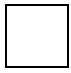
\includegraphics[scale=0.30]{img/QT6}\\
  \hline
 \end{tabular}
 \caption{Classification visuelle des cas d'arrêts et de récursions}
\label{tab:algo}
\end{table}


L'OcTree repose sur le même principe mais étendu à trois dimensions. Une cellule est donc découpée en huit parties à chaque fois.

\paragraph{Avantage de cette méthode}Cette structure est particulièrement intéressante pour la visualisation du pavage. En effet pour une fenêtre de visualisation donnée, il est très simple et rapide d'extraire la sous-arborescence correspondante à la fenêtre visualisée et permet aussi de ne pas afficher les objets trop petits. 

De plus il serait possible de créer une structure reposant sur le même principe que le QuadTree mais étant $k$-dimensionnelle\footnote{$k$ étant la dimension du problème fourni à \realpaver.}. Chaque espace peut alors être potentiellement subdivisé en $2^k$ sous-espaces. Cette structure permettrait d'éviter de recalculer l'arbre à chaque changement de variables de visualisation. On évite par ailleurs le cas de superposition de boîtes pour lequel l'algorithme n'est plus efficace (cf : figure \ref{fig:superpos}).
\begin{figure}[htbp]
\centering
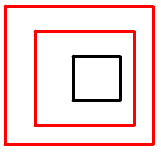
\includegraphics[scale=0.30]{img/QT8}
\caption{Superposition de boîtes}
\label{fig:superpos}
\end{figure}

\paragraph{Inconvénient de cette méthode}Le problème majeur de cette méthode se présente lorsque des boîtes sont côte à côte (cf : figure \ref{fig:frontiere}).
\begin{figure}[htbp]
\centering
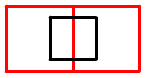
\includegraphics[scale=0.40]{img/QT7}
\caption{Superposition de boîtes 1}
\label{fig:frontiere}
\end{figure}
Dans une telle situation chaque division va entraîner la création d'un espace dans la même configuration. L'algorithme ne s'arrêtera donc pas avant d'avoir atteint la taille minimale d'un espace. Nous nous retrouvons donc avec un grand nombre de boîtes au niveau de ces \og frontières\fg{} (cf : figure \ref{fig:frontiere2}).
\begin{figure}[htbp]
\centering
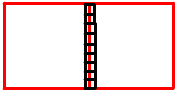
\includegraphics[scale=0.40]{img/QT9}
\caption{Superposition de boîtes 2}
\label{fig:frontiere2}
\end{figure}
Ainsi sachant que la précision maximale par défaut de \realpaver{} est de $10^{-16}$, cela implique qu'il est nécessaire d'au moins égaler cette précision pour l'arbre de visualisation. Ainsi pour une sortie de \realpaver{} contenant un total $l$ de longueurs de \og frontières \fg{}  cumulées et $p$ la précision du modèle, on a un nombre d'espaces à créer supérieur à $\frac{l}{p}$ avec $p$ très petit. Par exemple pour une sortie de \realpaver{} comportant une \og frontière \fg{} de taille $1$, il faudra au moins $10^{16}$ espaces pour la contenir. 

\paragraph{Brève conclusion} Le QuadTree est une structure intéressante pour la visualisation mais si un nœud de l'arbre a un coût en mémoire non nul, alors l'espace mémoire de la structure va exploser. Elle semble donc, pour le moment, inappropriée.

\subsection{\'Etude d'une seconde solution : le R-tree}
\paragraph{}Bien que le QuadTree soit une structure intéressante pour permettre l'indexation et la recherche de points dans un espace, celui-ci l'est beaucoup moins pour la gestion de données à dimensions non nulles. Le R-tree est une structure proposé en 1984 par Antonin \textsc{Guttman} permettant l'indexation et la recherche d'éléments de dimension $d > 0$ dans $k$ dimensions\cite{Guttman}.

\paragraph{}Le R-tree est une variante de l'arbre B, sa structure est la suivante :
\begin{itemize}
 \item Un noeud de l'arbre correspond à une boîte non-solution du pavage. Chacun de ces nœuds est un MBR\footnote{\og \emph{Minimum bounding rectangle}\fg{} : les rectangles étant, dans le cas présent, $d$-dimensionnels.} de ces fils.
 \item Chaque boîte peut contenir entre $m$ et $M$ sous-boîtes entièrement incluses. Avec $m\leq \frac{M}{2}$.
 \item Une feuille de l'arbre est une boîte ne contenant que des boîtes solution du pavage.
\end{itemize}

La figure \ref{fig:rtree} donne une bonne idée de l'organisation des R-trees :
\begin{figure}[htbp]
\centering
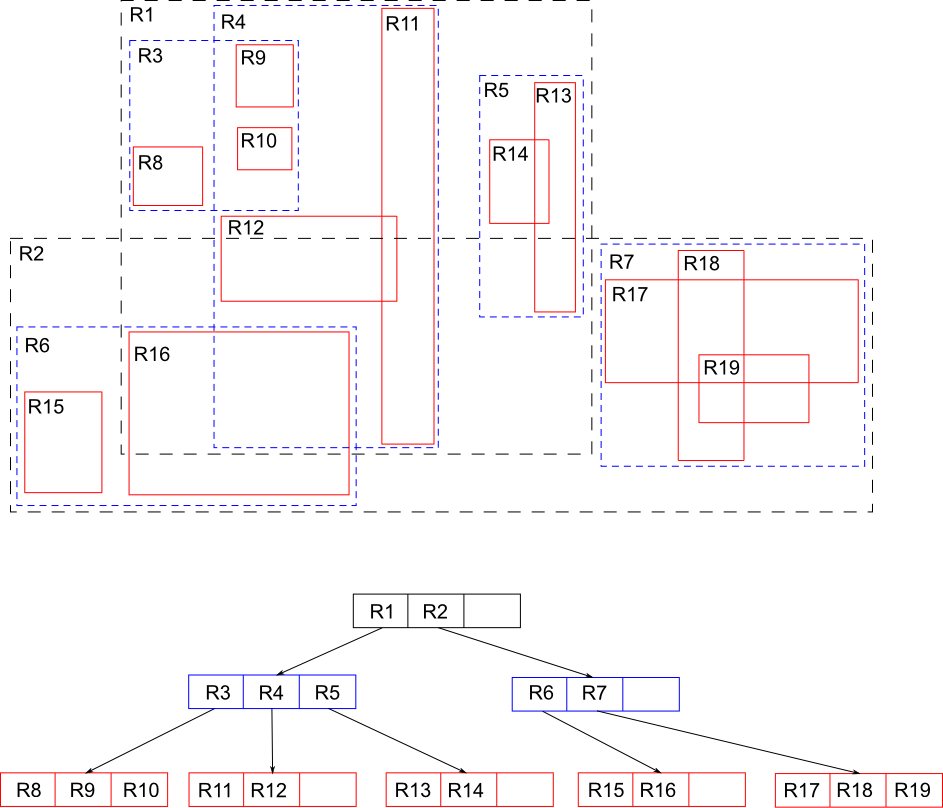
\includegraphics[scale=0.50]{img/rtree}
\caption{Représentation d'un R-tree\cite{wiki}}
\label{fig:rtree}
\end{figure}

Les algorithmes permettant la recherche et la création du R-tree sont quant à eux décrient dans l'article de \textsc{A. Guttman} dans la section \textbf{3. Searching and Updating}\cite{Guttman}. Nous rappelons brièvement les algorithmes de recherche (cf. Algorithme \ref{algo:recherche}) et d'ajout d'une boîte (cf. Algorithme \ref{algo:ajout}) \cite{poulos}. Il est important de noter que \textsc{Guttman} propose trois algorithme de \og split \fg{} qui permettent ensuite à l'algorithme de recherche d'être plus  ou moins efficace. Du moins efficace au plus efficace pour la recheche : un algorithme linéaire, un quadratique et un exponentielle.

L'algorithme \ref{algo:ajout} d'ajout présenté est implémenté avec le split linéaire.

\begin{algorithm}
\caption{\textbf{Recherche}(nœud $N$, rectangle $R$)}
/* \textit{Recherche l'ensemble des feuilles contenues dans un rectangle requête $d$-dimensionnel à partir d'un nœud $N$, les feuilles solutions seront stockées dans $\Lambda$} */
\label{algo:recherche}
\begin{algorithmic}[1]
\IF {$N$ n'est pas une feuille}
  \FORALL{éléments $n$ de $N$ dont le MBR intersecte $R$}
    \STATE \textbf{Recherche}($n$, $R$)
  \ENDFOR
\ELSE[$N$ est une feuille] %\COMMENT{$N$ est une feuille}
  \FORALL{éléments $n$ de $N$ dont le MBR intersecte $R$}
    \STATE ajouter $n$ à $\Lambda$
  \ENDFOR
\ENDIF
\RETURN $\Lambda$
\end{algorithmic}
\end{algorithm}

\begin{algorithm}
\caption{\textbf{Ajout}(élément $E$, nœud $NR$)}
/* \textit{Ajoute un nouvel élément $E$ dans le R-tree de nœud racine $NR$} */
\label{algo:ajout}
\begin{algorithmic}[1]
\STATE On parcourt l'arbre depuis la racine $NR$ jusqu'à la feuille appropriée. À chaque niveau, on sélectionne le nœud dont le MBR nécessite le plus petit élargissement pour contenir le MBR de $E$
\STATE En cas d'égalité, on choisit le nœud ayant le MBR de plus petite \og superficie \fg{}
\IF{la feuille atteinte $L$ n'est pas pleine}
  \STATE On insère $E$ dans $L$
  \STATE On met à jour tous les MBR de $L$ jusqu'à $NR$ pour qu'ils puissent contenir le MBR de E 
\ELSE[la feuille $L$ est pleine]
  \STATE On définie $\xi$ l'ensemble constitué de tous les éléments de $L$ et du nouvel élément~$E$\\
On choisit deux éléments $e_1$ et $e_2$ tel que la distance entre $e_1$ et $e_2$ soit la plus grande de toutes les autres paires de $\xi$\\
On crée deux nœuds $l_1$ et $l_2$ contenant respectivement $e_1$ et $e_2$
  \STATE On parcourt tous les éléments restants de $\xi$ et l'on assigne chacun d'eux à $l_1$ ou $l_2$, en fonction du MBR de ces nœuds qui permet le plus petit élargissement pour contenir le MBR de l'élément considéré
  \IF{égalité de l'élargissement}
    \STATE On assigne l'élément au nœud ayant le MBR de plus petite superficie
    \IF{égalité de superficie}
      \STATE On assigne l'élément au nœud ayant le moins d'élément
    \ENDIF
  \ENDIF
  \IF[On rappelle que m est le nombre minimal d'éléments que peut contenir un nœud]{il reste $\lambda$ éléments dans $\xi$ et qu'un nœud contient $m - \lambda$ éléments}
    \STATE On assigne tous les éléments restants dans $\xi$ à ce nœud
  \ENDIF
  \STATE On met à jour le MBR des nœuds se trouvant sur le chemin de $L$ à $NR$ pour que ceux ci couvrent le MBR de $l_1$ et $l_2$
  \STATE On effectue les \og splits \fg{} éventuels des nœuds supérieurs
\ENDIF 
\end{algorithmic}
\end{algorithm}


\paragraph{Avantages et inconvénients du R-tree} Le R-tree est une structure de données spécialement conçue pour la recherche de données à dimensions $d$ pour dans des espaces $k$-dimensionnels. L'arbre a une profondeur maximale $h_{max}$ égale à :
\begin{equation}
 h_{max} = \left\lceil\log_{m} n\right\rceil - 1
\end{equation}
et le nombre de nœuds est au pire égale à :
\begin{equation}
 \sum_{i=1}^{h_{max}}{\left\lceil\frac{n}{m^i}\right\rceil} = \left\lceil\frac{n}{m}\right\rceil + \left\lceil\frac{n}{m^2}\right\rceil + \cdots + 1
\end{equation}

 Bien que ne pouvant garantir de bonnes performances en pire cas\footnote{\og \emph{More than one substree under a node may need to be searched, hence it is not possible to guarantee good worst-case performance.}\fg{}\cite{Guttman}, section \textbf{3.1 Searching}}, le R-tree offre en pratique de bons résultats ; on pourra d'ailleurs se reporter à l'analyse de performances effectuer par A. \textsc{Guttman}\footnote{section \textbf{4. Performance}\cite{Guttman}}. Cependant il existe aujourd'hui de nombreuses variantes du R-tree ( R*tree, Hilbert R-tree, etc\dots{} ), on pourra donc, pour une analyse plus générale des différentes implémentations, préférer \og\emph{R-trees : Theory and Applications} \fg{}\cite{poulos}.

\subsection{Conclusion}
Au vu de l'étude comparative entre les deux structures, le R-tree nous semble une structure plus adéquate pour répondre à une visualisation des pavages. En effet, bien que le QuadTree soit adapté pour stocker des éléments sans dimension. Il devient moins performant et plus coûteux lorsque les éléments sont $d$-dimensionnels et notamment lorsque le pavage résultat possède un grand nombre de boîtes adjacentes comme c'est le cas pour la figure \ref{fig:DisqueDisque}. La structure R-tree quant à elle offre de meilleurs résultats sur les objets $d$-dimensionnels et semble donc plus adaptée pour notre logiciel de visualisation.
